% Created with jtex v.1.0.20
\documentclass{article}
\PassOptionsToPackage{short, nodayofweek}{datetime}

\input{curvenote.def}



% colors for hyperlinks
\hypersetup{colorlinks=true, allcolors=blue}
\hypersetup{
pdftitle={\@title},
pdfsubject={description},
pdfauthor={\@author},
pdfkeywords={},
addtopdfcreator={Written in Curvenote}
}

\usepackage{curvenote}

\title{CT scan reconstruction using machine learning}

\newdate{articleDate}{1}{1}{2024}
\date{\displaydate{articleDate}}

\author{\bfseries Luuk Froling\mdseries\\}

\begin{document}

\maketitle
\keywords{Finite volume, Direct current, Resistivity, DC equations}

\textbf{Author:} Luuk Fröling

\subsection{abstract}

abstract, work in progress

\subsection{Introduction}

\begin{itemize}
\item introduction x-ray
\item introduction ct scan
\item need for reconstruction algorithms
\item more advanced recon algo's -\textgreater  more computationally heavy
\item recent wave of breakthroughs in AI (attention is all you need)
\item how an iterative, computationally heave reconstruction algorithm can be sped up and how this relates to the RMS error
\end{itemize}

\section{Theory}

\subsection{Basics CT scans}

A computed tomography (CT) scanner is an imaging device that uses x-rays to create cross-sectional images of an object. It consists of an x-ray source and a detector placed at a distance from eachother. During scanning, both the source and the detector will rotate around the object to be imaged in steps. For each step, the source emits x-rays that pass through the object; the transmitted photons are measured by the detector. The number of detected photons at position i along the detector is given by:

\begin{equation}
\label{first }
\hat{y}_i  = N_0 \cdot \exp\left(-\int \mu(x, E) \, dx\right)
\end{equation}

where $N_0$ is the number of the x-rays emitted by the source, $\mu(x, E)$ is the linear attenuation coefficient and the integral in the exponent represents the cumulative attenuation along the x-ray path. $\mu(x, E)$ describes how many of the incoming x-rays are absorbed per unit of length, which depends on both the material of the object and the energy of the x-ray \citep{kamalian2016ct_principles}.

By rotating the source and detector around the object and recording measurements at multiple angles, a sinogram can be created. A sinogram is a 2D plot where each row corresponds to a detector reading at a specific projection angle.

\begin{figure}[!htbp]
\centering
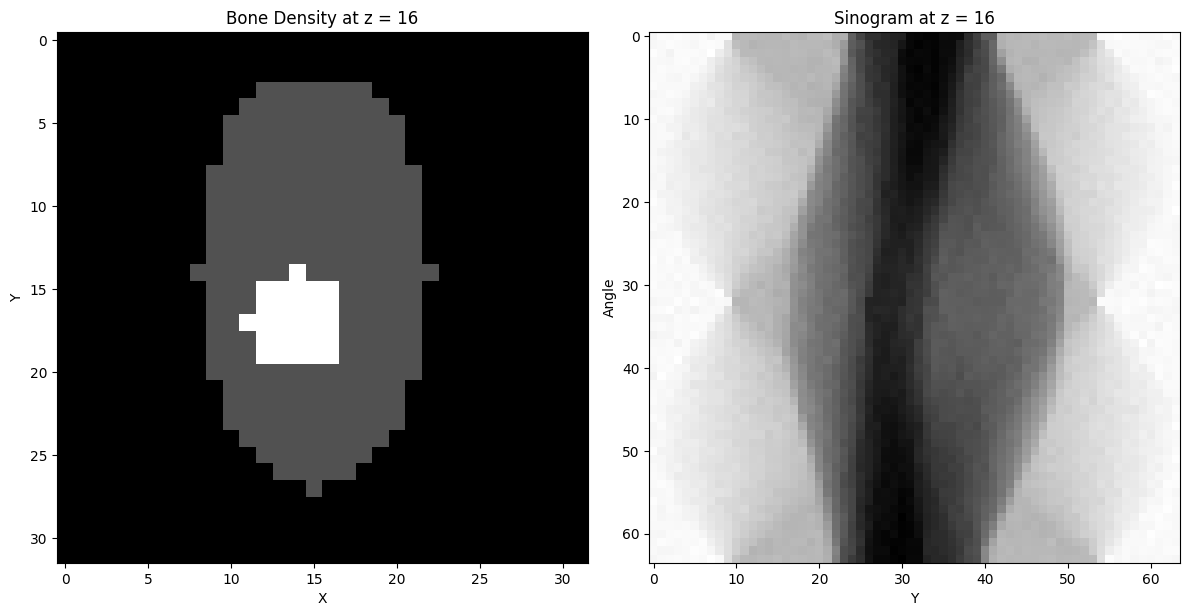
\includegraphics[width=0.7\linewidth]{files/3151776982ba6138bdf4c9ad99fa3c94.png}
\caption[]{\textit{left:} a 32x32 pixel phantom representing varying bone densities. \textit{right} corresponding sinogram with 64 projection angles. The lighter regions in the sinogram indicate higher photon counts. The CT energy used was [TODO].}
\label{phantomSinogram}
\end{figure}

A phantom and a corresponding sinogram can be seen in Figure~\ref{phantomSinogram}. The phantom is a 32x32 image, where each pixel represents a part of the phantom with a specific bone density. Lighter coloured areas having a higher bone density where darker areas have a lower bone density. On the right is the corresponding sinogram which consists of 64 measurements of $\hat{y}_i$ at different angles. The lighter parts of the sinogram correspond to more detected photons.

\subsection{Cone beam CT scan}

The sinogram in Figure~\ref{phantomSinogram} is true for a 1D detector, where we construct a single slice. A cone beam CT scan uses a source emitting x-rays in a cone-beam shape, which can be detected on a 2D flat-panel detector \citep{venkatesh2017cbct}.

\begin{figure}[!htbp]
\centering
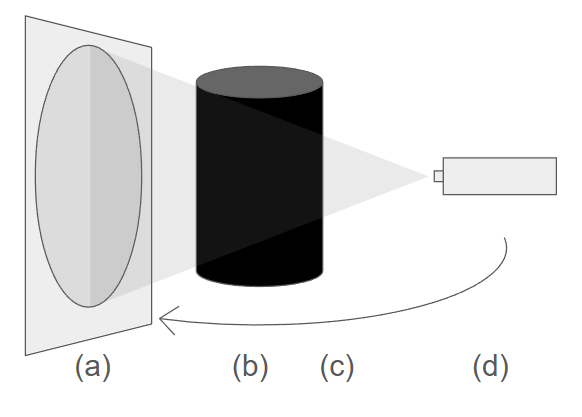
\includegraphics[width=0.5\linewidth]{files/cone_beam_ct-99b3680584828e6b48ebd5424f1fe103.png}
\caption[]{A schematic drawing of a cone-beam CT scan: (a) the 2D detector panel, (b) the phantom, (c) rotation direction of the source-detector pair (d) the x-ray source.}
\label{cone_beam}
\end{figure}

Figure~\ref{cone_beam} shows a cone beam CT scan setup, where both the detector and the source rotate around the object to acquire a set of 2D projection images at multiple angles. these measurements are known as rays.

The relationship between the object and the measured rays can be described by a projection matrix $A$. This matrix has dimensions $M \times N$ where $N$ is the number of voxels in the object and $M$ is the number of rays (measurements) collected by the detector. Each element $a_{mn}$ of the matrix is the contribution of the nth voxel of the object to be imaged to the mth ray of the detector \citep{Yang2017ProjectionMatrix}. The measured projections can thus be modeled as:

\begin{equation}
\label{projection_eq}
y = Ax
\end{equation}

where $x$ is the vectorised representation of the voxel values and $y$ contains the corresponding ray measurements. This formulation is will be used by the reconstruction algorithms during the simulations.

\subsection{Detector types}

Current CT scanners use an energy integrating detector (EID) \citep{marth2023photon}. An EID measures the intensity of the incoming x-rays by a two-step process: scintillation followed by photodetection. The scintillator will absorb the x-rays which have passed through the body and emit light in the visible spectrum. These re-emitted photons can be detected by photodetectors located underneath the scintillator. Due to the difference in energy of the incoming x-ray and the emitted visible light, multiple photons can be re-emitted. To measure a signal, EIDs integrate over time which loses all energy dependent information \citep{taguchi2013photon}.

\begin{figure}[!htbp]
\centering
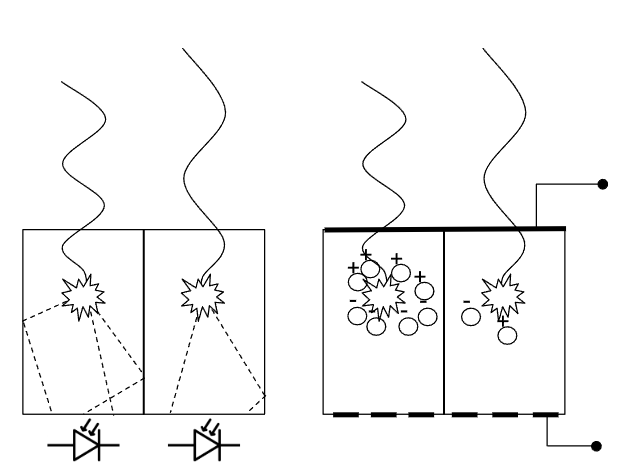
\includegraphics[width=0.5\linewidth]{files/detectorTypes-1f23300987a3b96a7f3effc6cb05b528.png}
\caption[]{\textit{left:} An EID where the incoming x-rays are absorbed within the scintillator. Several photons within the visible light spectrum are re-emitted which can be measured by the photodiodes located below the scintillator. \textit{right:} A PCD where incoming x-rays create electron-hole pairs in a semiconductor. This creates a current between the top and bottom of the semiconductor which can be measured by electrodes, preserving energy dependent information.}
\label{detectors}
\end{figure}

Photon-counting detector (PCD) CT scans improve the measurements by directly transforming the incoming CT scans into an energy-dependent signal which can be measured as illustrated in Figure~\ref{detectors}. The incoming x-rays will be absorbed in a semiconductor layer, forming electron-hole pairs which generate an electric signal proportional to the energy of the absorbed photon. Unlike EIDs, this allows the detector to retain energy-dependent information for each photon.

\begin{figure}[!htbp]
\centering
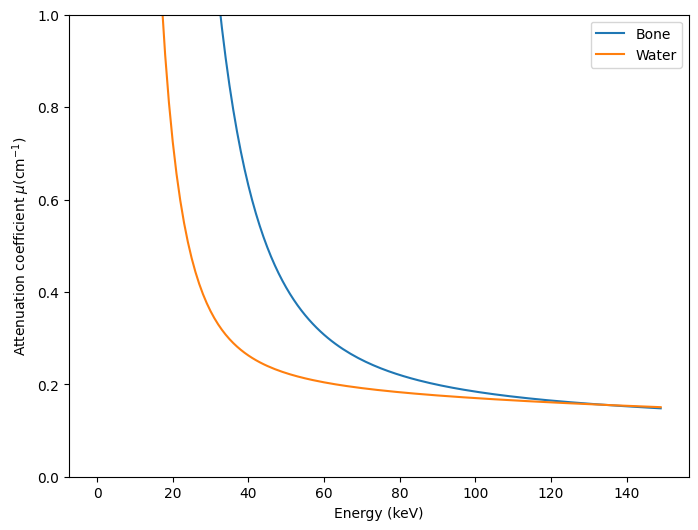
\includegraphics[width=0.7\linewidth]{files/64ccdbd7840b97b269bc4a429597ebd6.png}
\caption[]{The linear attenuation coefficient ($\mu$) of bone (blue) and water (orange) plotted as a function of the incoming x-ray photon energy. The different energy-dependent attenuation behaviour enables material differentiation in photon-counting CT.}
\label{matatt}
\end{figure}

The linear attenuation coefficient used in equation (\ref{first}) depends on the material and the x-ray energy used as illustrated by the attenuation curves in Figure~\ref{matatt}. Using a source emitting x-rays at a range of energies, energy bins can be generated by the PCD where each bin contains energy-specific measurements \citep{pcd2022}. This enables the differentiation between materials with similar densities which would otherwise appear similar in conventional CT scans using EIDs.

\subsection{Material decomposition}

Since different materials attenuate x-rays differently across the energy spectrum, PCD-CT can be used to distinguish between different tissue types within the body. To simulate this process and to describe the attenuation properties of different materials in a phantom, material decomposition is used \citep{mechlem2018joint}. In this work, material decomposition models each material in the phantom as a linear combination of two basis materials: bone and water.

The reconstructed image of a PCD CT scan will therefore consist of 2 images, one displaying the bone density and one displaying water density. The linear attenuation coëfficient of any material within the phantom can then be described as:

\begin{equation}
\label{muE}
\mu(E) = \sum_{b=1}^{B} A_b f_b(E)
\end{equation}
where $A_b$ is the line integral of material b and $f^b(E)$ describes the attenuation coefficient of the basis material b. Combining equation (\ref{first}) and (\ref{muE}) gives an expression for the photon count at the detector:

\begin{equation}
\hat{y}_i = \int_0^{\infty} \phi_{\text{eff},i}(E) \exp\left( - \sum_{b=1}^{B} A_b^i f_b(E) \right) \, dE
\end{equation}

where $\phi_{\text{eff},i}(E)$ is an effictive x-ray spectrum which includes all source and detector effects.

\subsection{Projection algorithms}

To view the cross-sectional image of an object from these measurements, either from a detector or from simulations using equation (\ref{projection_eq}), a reconstruction algorithm needs to be used. The simplest form of a reconstruction algorithm is a backprojection algorithm; during reconstruction, the algorithm spreads each projection back across the image plane along the same angle it was acquired. This often leads to blurry images as the intensity is spread along lines rather than concentrated at specific points \citep{zeng2001image}. Backprojection works primarily for single energy CT scans as illustrated in Figure~\ref{phantomSinogram}, however it can be used for dual-energy CT scans by a two-step image based method. The first step is to reconstruct an image for each energy bin and these intermediate images are then decomposed into material-dependent images \citep{mory2018comparison}.

The two-step, image based method has several drawbacks. First, beam hardening artifacts often occur as the attenuation coefficient is still averaged over a line. Secondly, the first step leads to a loss of information as there is no one-to-one mapping between the projections and the images. The second step is unable to compensate for this loss as it has no access to the photon counts. Recently one-step methods have been proposed which reconstruct material-specific images directly from photon counts \citep{mechlem2018joint}. These are all iterative methods as no analytical inversion formula exists.

Import parameters of the interative algorithm introduced are the data attachment term and the cost regularisation. The data attachment term ensures the reconstructed material images explain the measured photon counts and the regularisation term enforces smoothness or prior knowledge on the material images \citep{Zhang2018Regularization}, a cost function can be defined which includes both terms. The iterative algorithm reconstructs an image for each material and compares the image to the measurements using the cost function and updates the images accordingly.

A downside to the iterative algorithm is the computational time. For each iteration there is a forward projection and a backprojection, as well as an error calculation. There is also a large amount of iterations needed to get to an accurate solution. This work will look at including machine learning to replace the iterative steps.

\subsection{Machine learning - Neural networks}

Neural networks are a subset of machine learning and play a crucial role in deep learning algorithms. A simple, fully connected neural network consists of nodes stacked in layers: an input layer, one or more hidden layers and an output layer.

\begin{figure}[!htbp]
\centering
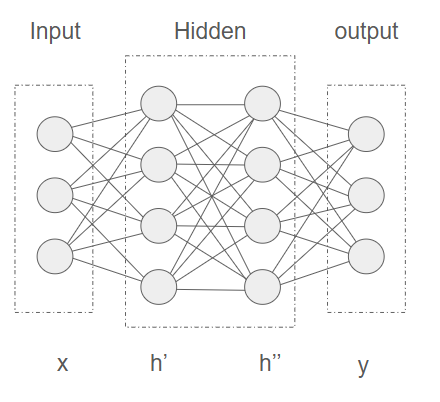
\includegraphics[width=0.7\linewidth]{files/neuralnetwork-7c664ffdc7b4a7b98a97346c5a4ef4fb.png}
\caption[]{A neural network consisting of 3 input nodes, 2 hidden layers with 4 nodes each and an output layer with 3 nodes. The input values are represented by an array x, the hidden layers by array h' and h'' and the output layer by y.}
\label{neural_network}
\end{figure}

All nodes in a layer are connected to an adjacent layer by weigths. Figure~\ref{neural_network} shows a simple neural network, where input layer x and first hidden layer h' are connected by a matrix of weights $W_1$, the states of the first hidden layer can be calculated as

\begin{equation}
\label{denseLayer}
\mathbf{h}_1 = \sigma(\mathbf{W}_1 \mathbf{x} + \mathbf{b}_1)
\end{equation}
with $\mathbf{W}_{1,nm}$ representing the weight connecting the m-th input neuron to the n-th neuron in the first hidden layer, and $\sigma$ is an activation function (e.g., sigmoid or softmax) that scales the output between 0 and 1 to stabilise the network. Equation (\ref{denselayer}) can be repeated for every following layer where the output of a layer is used as an input to calculate the following layer.

Neural networks learn by backpropagation. Backpropagation looks at the error between the output of the network and the desired output. This error is generally propogated backwards through the network by looking at how each weight needs to change to minimise this error.

\subsection{Machine learning - Convolutional neural network}

A convolutional neural network (CNN) can be used to more accuratly extract features from images for processing. A CNN consist of a kernel (also called a filter) and one or more channels. The kernel is smaller than the input data but has the same number of dimensions (e.g., 2D for 2D images). The kernel contains weights that are learned during training.

The kernel is moved across the input data, performing element-wise multiplication with the region of the input it covers, followed by a sum. This operation extract features such as edges, textures and shapes \citep{yamashita2018convolutional}. We can write the output feature map of a convolutional layer as

\begin{equation}
S(i, j) = (\mathbf{K} * \mathbf{X})(i, j) = \sum_m \sum_n \mathbf{K}(m, n) \cdot \mathbf{X}(i + m, j + n)
\end{equation}

where $(i,j)$ are spatial indices, $\mathbf{X}$ the relevant kernel and m and n the kernel sizes. After a convolution layer, $S(i, j)$ can be either vectorised to be used as an input for a fully connected layer as described in equation (\ref{denseLayer}) or used as an input for a second convolution layer.

\begin{figure}[!htbp]
\centering
\begin{verbatim}
Text(0, 0.5, 'Y')
\end{verbatim}

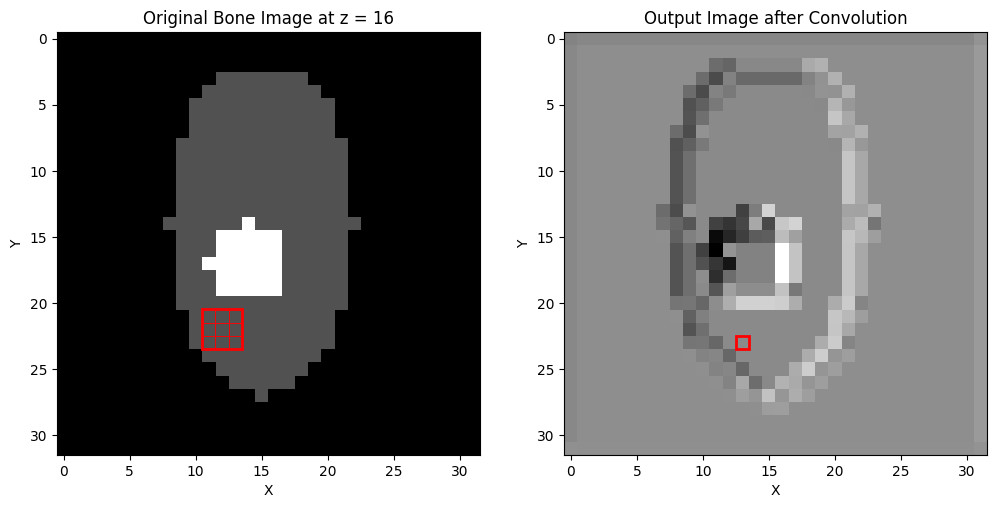
\includegraphics[width=0.7\linewidth]{files/df9eecf15dc213c5837add0b2c07a681.png}
\caption[]{\textit{left :} original phantom with a 2D 3x3 randomly initialised kernel drawn on top. each individual square represents a pixel, with the outer square representing the kernel. \textit{right :} phantom after 2D convolution layer has been applied.}
\label{convex}
\end{figure}

The left part of Figure~\ref{convex} shows a 3x3 convolution kernel (red) placed on a phantom and the right part of the figure shows the imgage of the phantom after the convolution. Even with randomly initialised weights, there is already an edge-detection like pattern.

A CNN typically consists of multiple layers stacked on top of each other, allowing deeper feature extraction. Early layers can detect simple features like edges, while deeper layers can detect more complex structures like shapes and objects.

\subsection{Machine learning - U-Net architecture}

Multiple convolution layers can be combined to form an encoder. An encoder reduces the size of the image between each layer using a max pool layer.A max pool layer devides the input into rectangular regions and taks the maximum value from each region, reducing the image size and allowing the network to capture more abstract and higher-level data.

Similarly a decoder can be used to an abstract representation and generate an output image. A decoder uses deconvolution layers which increases the size of the image as more features are added back in.

\begin{figure}[!htbp]
\centering
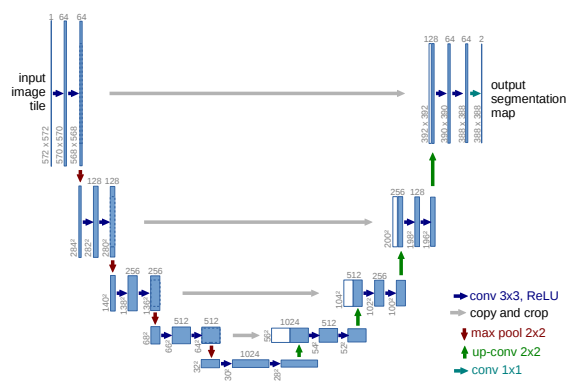
\includegraphics[width=0.75\linewidth]{files/Unet-b453ddb3b21672f27228e873588d59c4.png}
\caption[]{A U-Net architecture for an image with a 32x32 lowest possible resolution. Each blue square represents a multi-channel feature map with the amount of channels denoted on top of the box. Gray arrows represent cross over layers with the white boxes representing copied layers from the encoder \textit{Figure reproduced from} \citep{oktay2018attention}}
\label{unet}
\end{figure}

Figure~\ref{unet} shows a U-Net architecture, which combines an encoder and a decoder with an equal amount of layers. Between each layer of the encoder and decoder part of the network, there is a skip-connection layer as well which copies the feature map from the encoder layer to the decoder layer. This allows the decoder to use features which might have been lost while encoding the image.

\subsection{Machine learning - Attention gate}

For feature extraction from images where both local and non-local features are of importance, convolution layers can be combined with attention mechanisms. An attention mechanism is a technique used in machine learning used to allow machine learning models to attend to the most relevant parts of the input data \citep{vaswani2017attention}.

An attention mechanism takes the input vector $x_{i}^{l}$ and multiplies it by an attention score $\alpha_{i}^{l}$ to perserve only the activations relevant to the task. To calculate $\alpha_{i}^{l}$,  an intermediate attention score $q_{\text{att}}^{l}$ (the attention score $q_{\text{att}}$ for layer l) can be defined as
\begin{equation}
q_{\text{att}}^{l} = \psi^{T} \, \sigma \left( W_{x}^{T} x_{i}^{l} + W_{g}^{T} g_{i} + b_{g} \right) + b_{\psi}
\end{equation}
where $g_{i}$ the gating feature vector, $W_{x}^{T}$ and $W_{g}^{T}$ weight matrices similar to those used in equation (\ref{denseLayer}), $\psi^{T}$ another linear transformation and $\sigma$ an activation function. The final attention coefficient $\alpha_{i}^{l}$, the final attention mask that says which parts of the feature map should be passed forward, is then calculated as

\begin{equation}
\alpha_{i}^{l} = \sigma_{2} \left( q_{\text{att}}^{l}(x_{i}^{l}, g_{i}; \Theta_{\text{att}}) \right)
\end{equation}
with {\textbackslash}Theta\_\{{\textbackslash}text\{att\}\} representing the learned parameters of the attention block: all weights and biases. The final output of the attention gate it

\begin{equation}
\tilde{x}_i^l = \alpha_i^l \cdot x_i^l
\end{equation}

where regions get $\alpha = 1$ where less important regions get $\alpha \approx 0$

\subsection{Machine learning - Attention U-Net}

Attention mechanisms can be added to the skip-connections of the U-Net model in Figure~\ref{unet}, allowing the network to focus on non-local features during the reconstruction of the image. The combination of attention mechanism and convolutional layers can be used to recognise certain features like edges and to make connection between features in different parts of the image \citep{oktay2018attentionunet}.

\begin{figure}[!htbp]
\centering
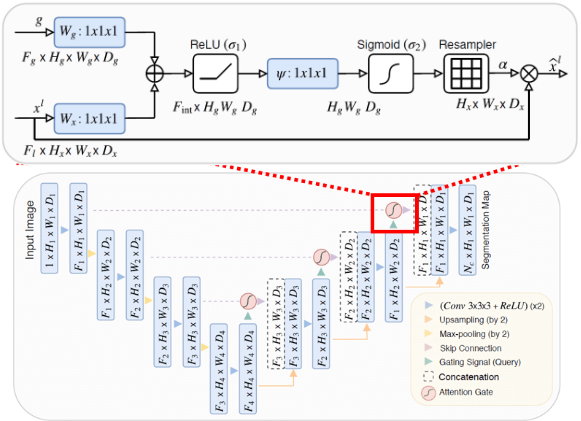
\includegraphics[width=0.7\linewidth]{files/AttU-Net-86c6f656da029e6df27f6848620cbcbe.png}
\caption[]{Schematic overview of a U-Net model with attention gates added to the skip-connections. The inset (top) shows a zoomed-in view of an attention gate, the gating signal $g$ is taken from the previous decoding layer and the input $x^l$ is the skip-connection layer. \textit{Figure reproduced from} \citep{oktay2018attentionunet}}
\label{attunet}
\end{figure}

The gate vector $g$, also called the gating signal, for each skip-connection layer connects the output of the previous decoder layer to the skip-connection input vector. This is illustrated in Figure~\ref{attunet}. //Work in progress

For each skip connection the output of the previous decoder layer is used as a gating signal $g$. //Work in progress

\begin{figure}[!htbp]
\centering
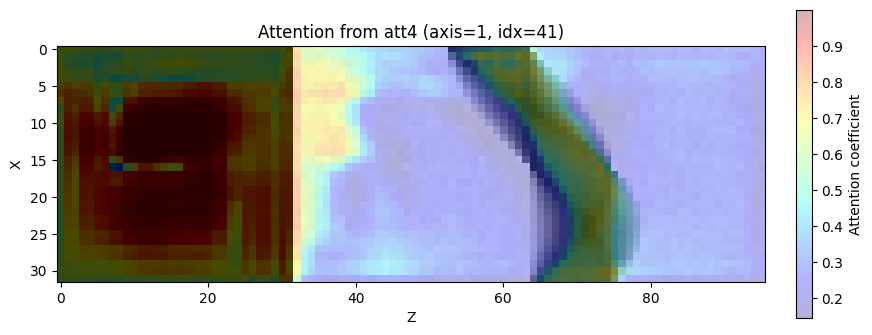
\includegraphics[width=0.7\linewidth]{files/61e001e87d8f0264596b2282806f90e4.png}
\caption[]{An attention map showing how an attention mechanism can be used to have the model focus more on important features, which in this case is the sinogram.}
\label{attention_network}
\end{figure}

Figure~\ref{attention_network} shows an attention map from a AttU-Net model trained on CT scan reconstruction. An attention map has been drawn to illustrate $\alpha_{i}^{l}$ for the first skip-connection. For this specific application it is as expected the attention gate focuses on the lower-intensity parts of the sinogram as these areas provide the most information about the imaged object.

\section{Method}

\subsection{Generating phantoms}

The phantoms, as illustrated in Figure~\ref{phantomSinogram}, are randomly generated according to a set of rules:

\begin{itemize}
\item each phantom is 32x32x32 pixels and consists of 2 channels, one for bone and one for water.
\item each phantom has a main, elliptical body centered in the image consisting of a low mass density of both water and bone
\item The center of the body can be randomly offset by -3 to +3 pixels in both the x and y directions (uniform distribution).
\item The size of the main body varies, with the distance between the points on the axis varying between 1 and 3 pixels uniformly distributed.
\item Each phantom has 2 internal features, represented as smaller elliptical regions within the main body.
\item Each feature has either a higher bone density or a higher water density than the other.
\item The bone and/or water density cannot be lower in a feature than the main body
\end{itemize}

Each feature represents a distinct elliptical region. Because photon counting detectors (PCDs) allow differentiating tissue types, we assign one feature a higher bone density and the other a higher water density. This design ensures that the network is trained on a task relevant to the clinical use of PCDs. These rules have been implemented in python to generate a sample of phantoms as seen in the supporting notebooks.

Due to constraints within the iterative reconstruction algorithm, the bone and water densities of the features are restricted to be higher than those of the main body.

\subsection{acquiring data}

A machine learning model will be trained to use information from sinogram space to adjust images in image space. The network will be trained to perform this conversion in iterative steps similar to an iterative reconstruction method \citep{mechlem2018joint}.
First, for a set of phantoms detector measurements will be simulated with x-rays at multiple energy levels: ... kV, ... kV and ... kV. These measurements are done with 32 projections per phantom. An example phantom can be seen in Figure~\ref{phantomSinogram}, with a corresponding sinogram. (which energies?).

Next, each set of detector measurements will be reconstructed using the iterative algorithm with 40 iterations. These iterations will be used to construct input-output pairs for training the model. Using a stride, the input is defined as the image from the nth iteration, with a corresponding output image taken from the (n+stride)th iteration.

Using a stride between input and output images allows the model to learn from a wider variety of scenarios within the same training time. In this work, a stride of 4 is used. This work made use of ... phantoms, which generated ... input-output pairs using a stride of 4 .

\subsection{Attention based UNet}

To enable the network to learn how features in the image space and the projection (sinogram) space attend to eachother, a U-Net architecture with attention mechanisms integrated into the skip connections is used (AttU-Net) as described by \citep{oktay2018attentionunet}. The attention gates help the model to focus on which parts of the sinogram contribute to specific image regions.

The AttU-Net model is illustraded in Figure~\ref{attunet}. The architecture consists of five convolutional encoder blocks, a bottleneck block, and five decoder blocks. The number of channels increases through the encoder (64, 128, 256, 512 and 1024), and then decreases symmetrically through the decoder. The output layer applies a sigmoid activation to produce voxel-wise probabilities.

The model is trained on an NVDIA Tesla A100, with 4 hours allocated per run. In total 6 runs were completed. The model uses MSELoss as a loss function and Adam optimisation, which is a stochastic gradient descent method. The learning rate is set to 0.001, which is commonly used with Adam optimisation \citep{kingma2014adam}.

\subsection{shaping the data}

The AttU-Net model takes an image as input and produces an image of the same size as an output. Sice 2 different images are used (the image and the projection), these must be combined into a single matrix. The projection has dimensions he projection matrix will have the dimensions ( number of projections) x (z pixels detector) x (y pixels detector), where this work uses 32 projections and a detector of 64 by 44 pixels as set for the simulations in the supporting notebooks.

Aditionally, due to the pooling layers all dimensions must be powers of 16 as to not get an uneven amount of devisions. The projection matrix is originally 32 x 44 x 64 pixels, which we can pad with zeros to 32 x 48 x 64 pixels. The image will is 32 x 32 x 32 pixels which we can pad to 32 x 48 x 32 to fit the dimensions of the projections. The final input set to the network will be 10 x 32 x 48 x 96 as we use 10 channels in total.

\section{results}

\subsection{Visualisation reconstruction}

During evaluation the model has been run on 20 validation sets generated under the same conditions and rules as those used for training. By taking the first image from the iterative algorithm, 20 reconstructions can be made using the proposed AttU-Net model.

\begin{figure}[!htbp]
\centering
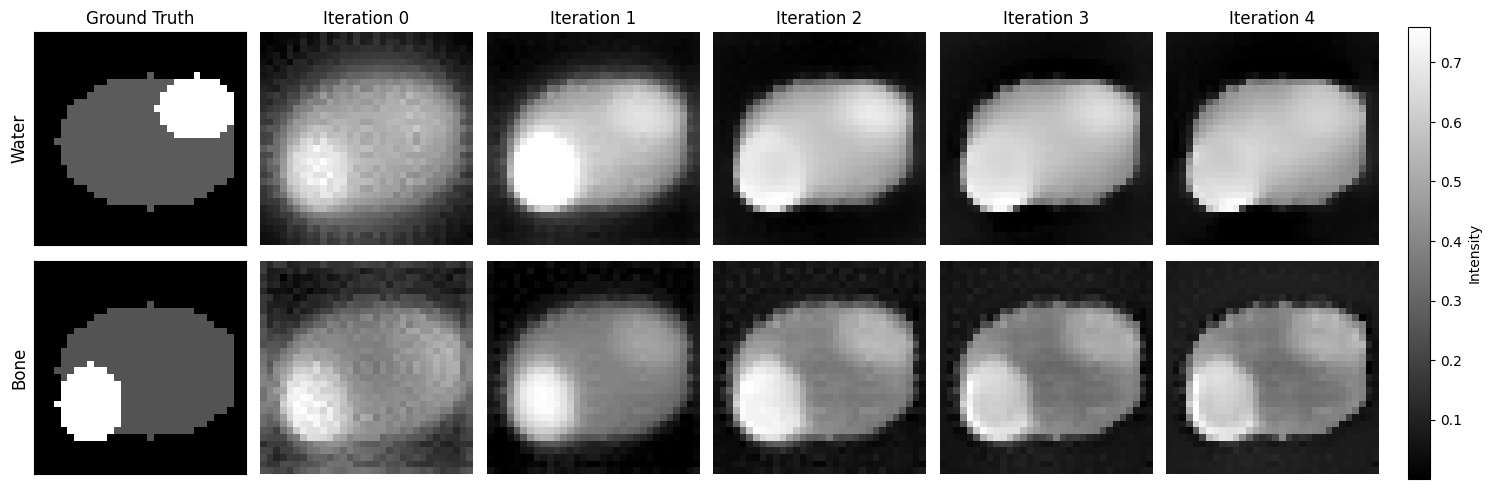
\includegraphics[width=0.7\linewidth]{files/7919280d54a67f0898be36384abd7990.png}
\caption[]{Top row (water), left to right: Ground truth (GT) water image; iteration 0 (first reconstruction) from iterative algorithm; subsequent reconstructions by the model.
Bottom row (bone), left to right: GT bone image; iteration 0 (first reconstruction) from iterative algorithm; subsequent reconstructions by the model.}
\label{bone_recons}
\end{figure}

The first 5 reconstructions of the second phantom are displayed in Figure~\ref{bone_recons} and the first column displays the ground truth (GT) images as a reference. The rows show the reconstruction process using the model for water and bone respectively, where each column is an iteration. In the GT images, distinct features are visible: a bone structure in the lower left quadrant and a water structure in the top right quadrant. These serve as reference to evaluate the reconstruction quality.

The first reconstruction shows that the AttU-net model accuratly recongnises the key features of the phantom, however the water feature is faint in the water density image. As reconstruction progresses, the overall water density increases while the edges between distinct features of the phantom are blurred. The bone density image looks to converge to a state where the phantom has a lower density, with both water and bone features present.

\subsection{Visualisation comparison}

To better understand the quality of the images compared to the iterative algorithm, the iterative algorithm has been used to reconstruct the phantoms as well using the same parameters as used during training.

\begin{figure}[!htbp]
\centering
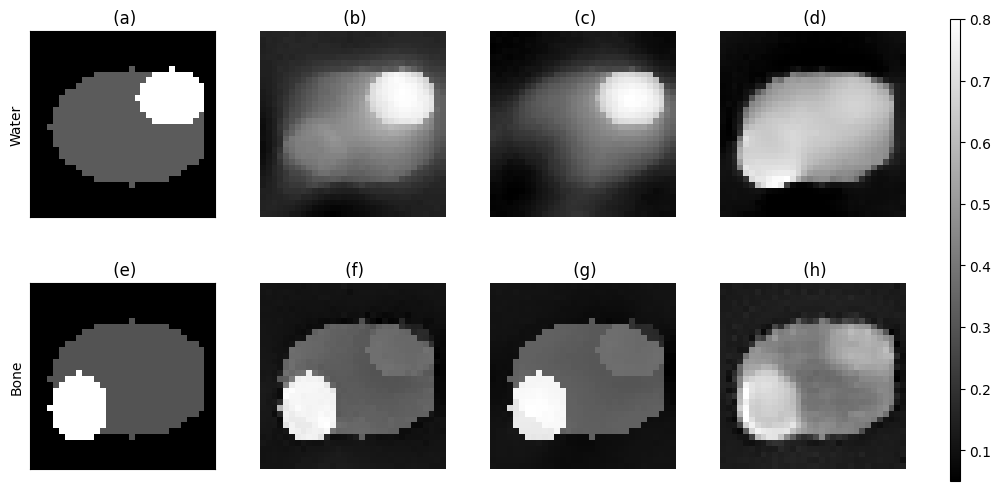
\includegraphics[width=0.7\linewidth]{files/afec7fb8a942be43385875429673a4f0.png}
\caption[]{(a) GT water image (b) smallest RMS water image iterative algorithm (c) water image from last iteration iterative algorithm (d) water image reconstructed by the model after 3 iterations (e) GT bone image (f) smallest RMS bone image iterative algorithm (g) bone image from last iteration iterative algorithm (h) bone image recontructed by the model after 3 iterations.}
\label{reconPhantom}
\end{figure}

Looking at the reconstructions corresponding to the smallest root mean square (RMS) error across all iterations (panel b and f), both water and bone features are present in their respective images. However the iterative algorithm does not fully distinguish between the two features, as the water feature can be faintly seen in the bone images and vice versa. For the final iteration of the iterative algorithm (panel c and g), the water image shows a clear reduction of the bone feature. This indicates an overcompensation compared to panel b.

The images reconstructed by the model after 3 iterations are shown in panel d and h. The water shows a nearly constant value throughout the entire phantom, unable to distringuish any features. The bone image clearly shows where the bone feature is located.

\subsection{RMS over time}

By calculating the root mean square (RMS) error at each iteration for both the iterative algorithm and the model with the ground truth (GT) image, we can compare reconstruction error as a function of time.

\begin{figure}[!htbp]
\centering
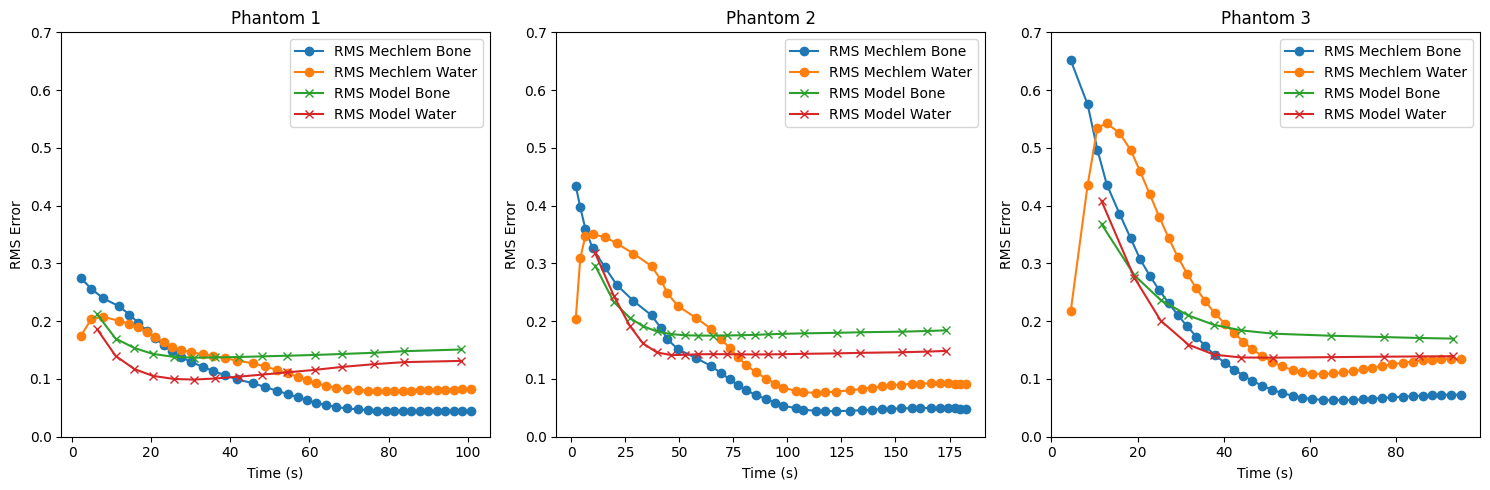
\includegraphics[width=0.7\linewidth]{files/586fa19a8938bf6fcb255a7e08c69611.png}
\caption[]{RMS error over time for three phantoms reconstructed using both the iterative method (orange: water; blue: bone) and the proposed model (red: water; green: bone).}
\label{rmsTime}
\end{figure}

Figure~\ref{rmsTime} shows the RMS error over time for bone and water images reconstructed by both methods for 3 phantoms. The model has been cut off after the iterative algoritm stopped running for phantom 1 and 3. In all three cases, the model achieves a lower initial error but converges to a bigger error compared to the iterative algorithm. For both algorithms the RMS error of the water images converges to a higher value than the RMS of the bone images.

\begin{figure}[!htbp]
\centering
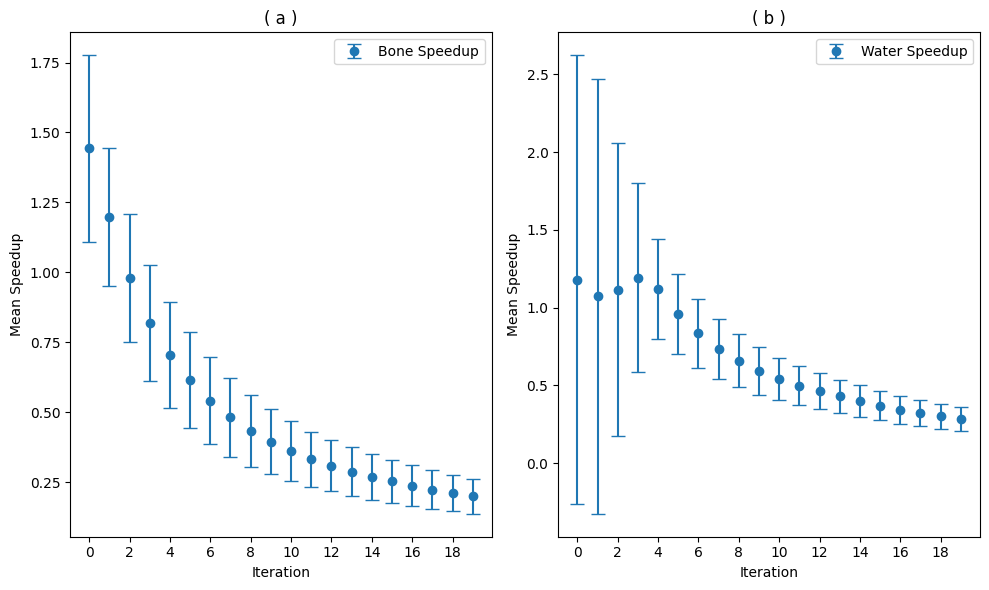
\includegraphics[width=0.7\linewidth]{files/2736d68d407f8ad6de225a7e5df53bf4.png}
\caption[]{The RMS-error plotted against time for 3 phantoms reconstructed using both the iterative method as well as the model. For both methods, the RMS is calculated for the bone and water image.}
\label{speedup_interpolated}
\end{figure}

Looking at a dataset of 20 phantoms, the average time taken for the first iteration of the model is 9.3 seconds with a standard deviation of 1.5 seconds. The average speedup for bone for this step (how long it takes the iterative algorithm to get to the same RMS error) is 1.44 times, or 44\% while the average speedup for water is 1.17 times, or 17\%. As the average time per iteration has a standard deviation of 1.5 seconds, the average speedup can be plotted against iteration of the proposed model as illustrated in Notebook-code.

\subsection{wrong reconstructions}

potentially display another set of reconstructions which are not good to highlight the inconsistency in the training data

\section{Discussion}

\subsection{non-machine learning speedup}

\begin{itemize}
\item pytorch is highly optimized, mechlem is not
\item
\end{itemize}

\subsection{pixel size and number of projections necessary}

There will not be a linear relationship between the amount of projections necessary and the amount of pixels in the image. will this have an impact?

\subsection{Model is only as good as your data}

Looking at the accuracy of the model

\subsection{Adding cross attention between spaces}

\begin{itemize}
\item adding cross attention can more accuratly predict which part of the sinogram attend to which parts of the image. Then convolution can still be used to reconstruct the image.
\end{itemize}

\section{Conclusion}

\clearpage
\bibliography{main.bib}

\end{document}
